
In summary we generate a series of training data for the specified earthquake based on different Q-factor parameters. For each station we train a set of neural networks. In an optimization process, we compute a set of parameters that provide the best match with observation. Then we peak the mean value of the observation Q equation and find the closes value to it from training data. We exclude that value from training data and use it as a target value in optimization process. According to the results we pick those velocity ranges that the synthetic optimization test could find the accurate results for them and also the points are in the one standard deviation of the results. Fig.~\ref{fig:Figure_1} represents the processing steps. 

 \begin{figure}
    \centering
    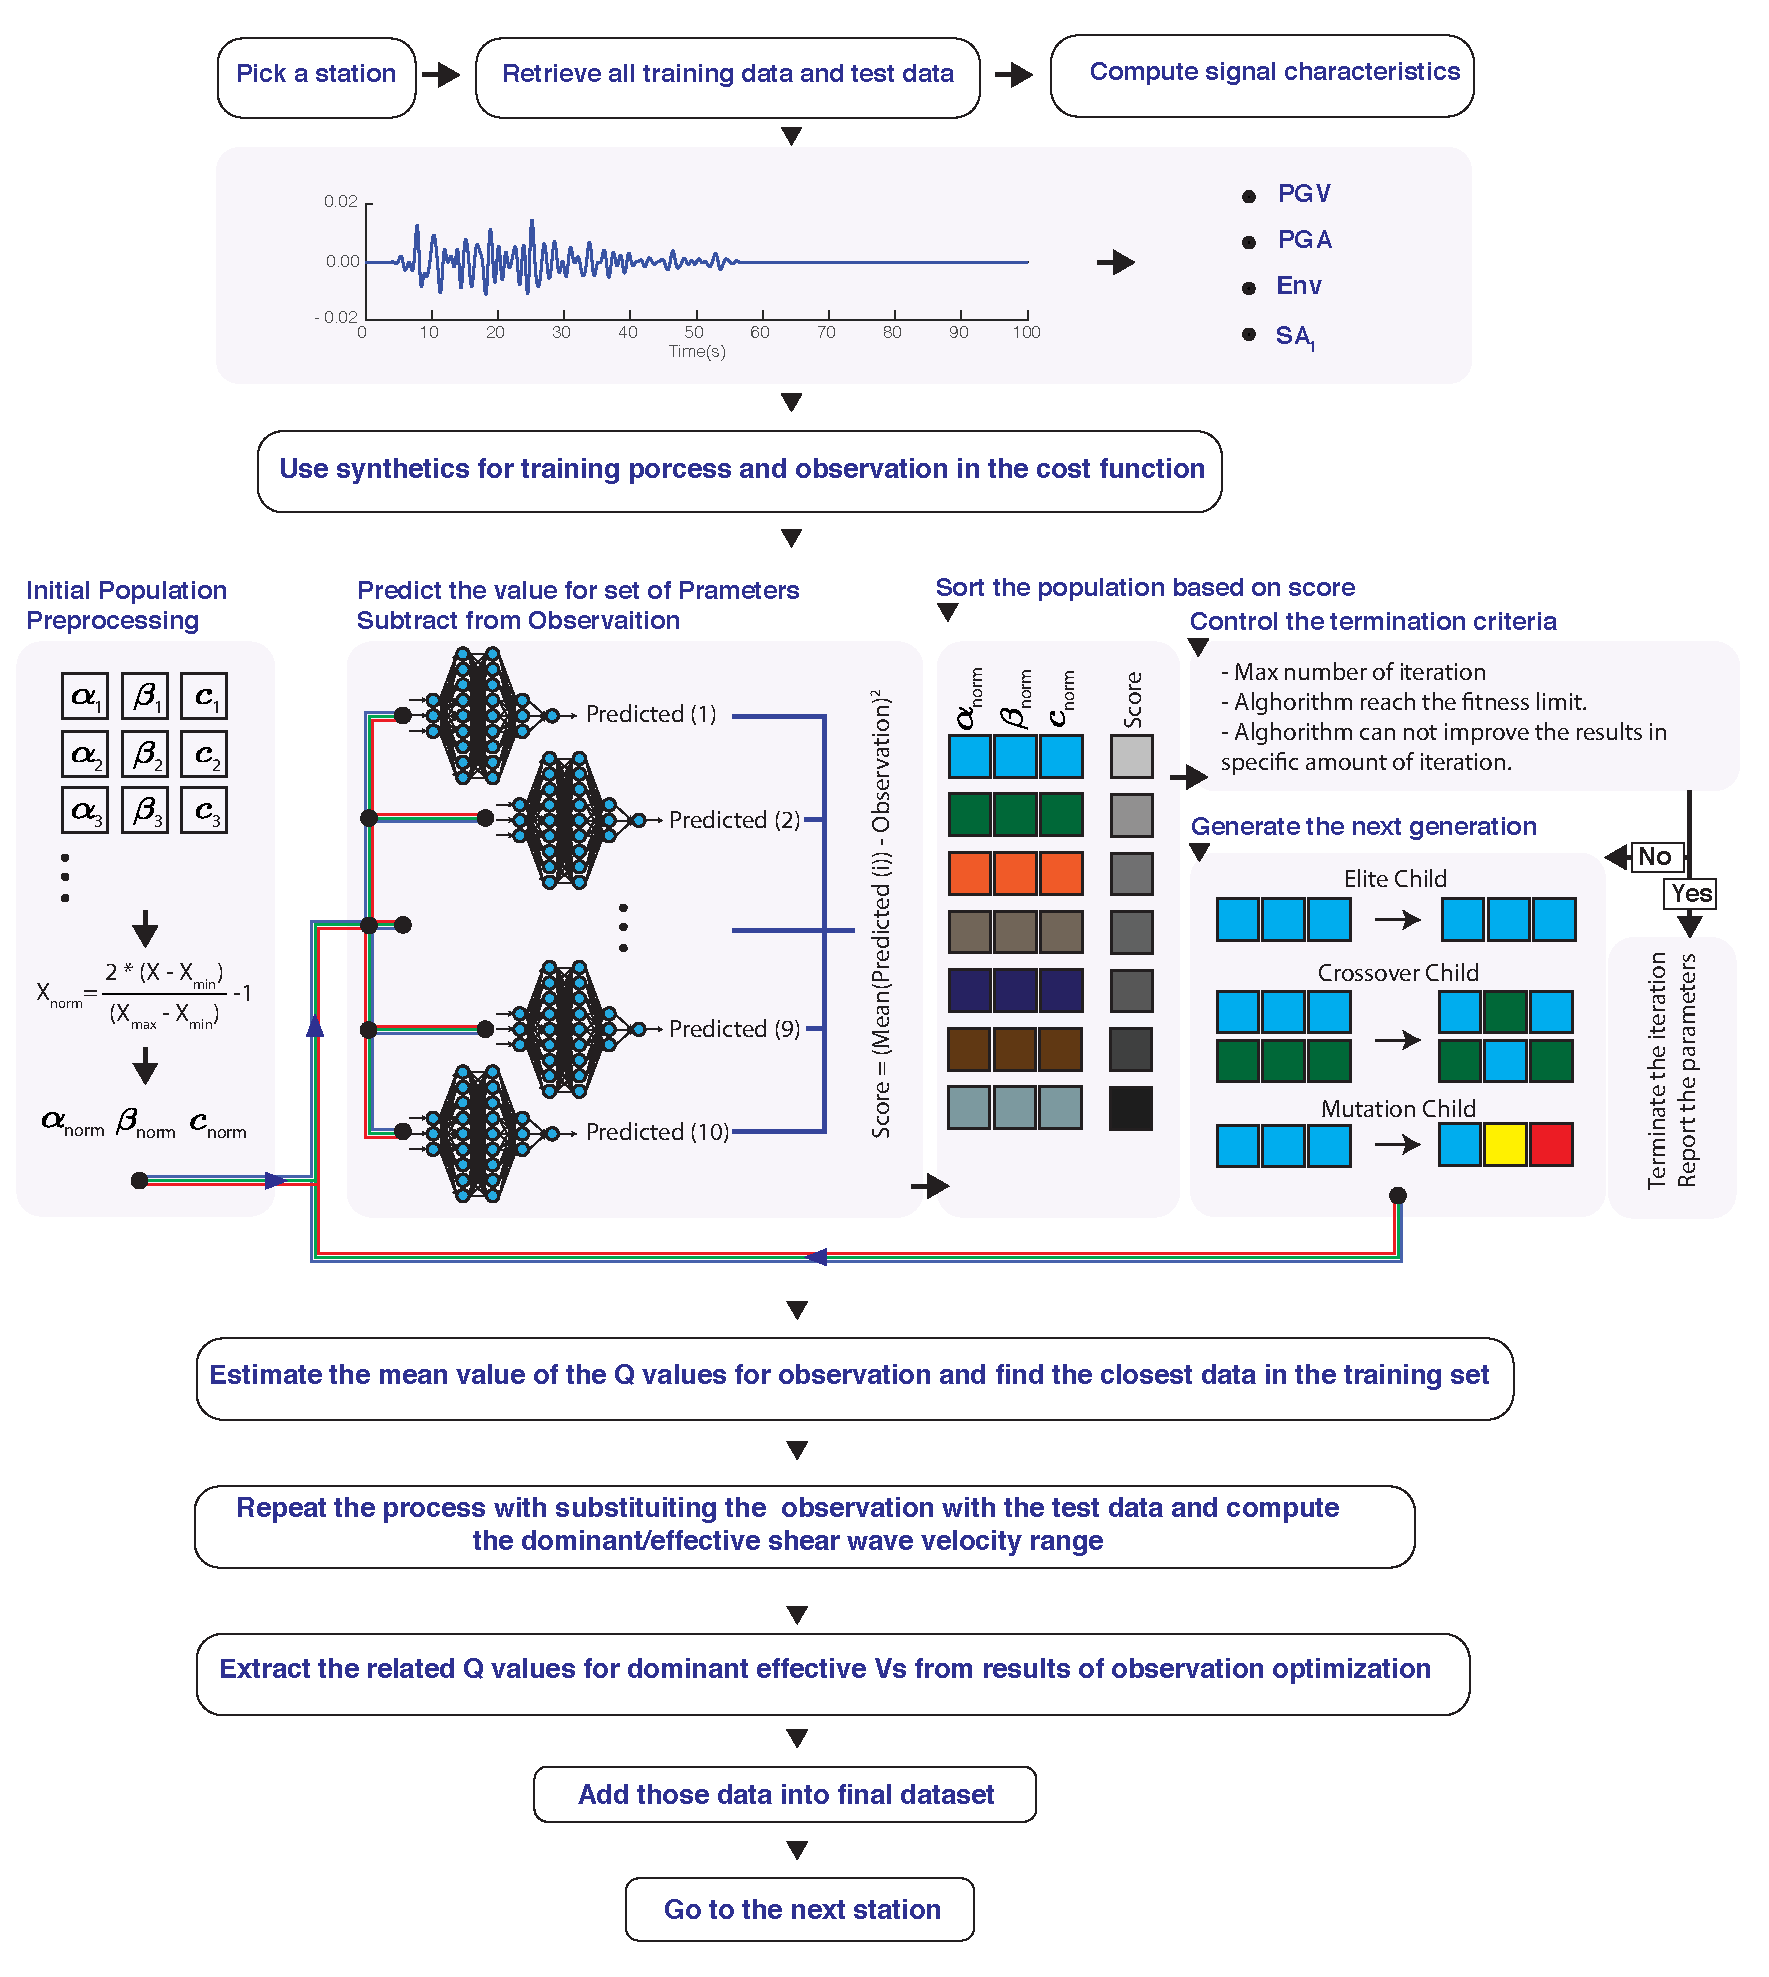
\includegraphics[width=\textwidth]{figures/pdf/Figure_1.pdf}
    \caption{Processing steps}
    \label{fig:Figure_1}
\end{figure}




